% ball.tex -- The smallest enclosing ball: an undergraduate introduction.
% Build:  pdflatex ball.tex   (twice, for the references)
%    or:  tectonic ball.tex

\documentclass[11pt,a4paper]{article}

\usepackage[T1]{fontenc}
\usepackage[utf8]{inputenc}
\usepackage{amsmath,amssymb,amsthm}
\usepackage{mathtools}
\usepackage{booktabs}
\usepackage{tikz}
\usepackage{listings}
\usepackage[margin=3cm]{geometry}
\usepackage[colorlinks=true,linkcolor=blue!50!black,citecolor=blue!50!black,urlcolor=blue!50!black]{hyperref}

\usetikzlibrary{calc}

\theoremstyle{plain}
\newtheorem{theorem}{Theorem}[section]
\newtheorem{proposition}[theorem]{Proposition}
\newtheorem{lemma}[theorem]{Lemma}
\newtheorem{corollary}[theorem]{Corollary}
\theoremstyle{definition}
\newtheorem{definition}[theorem]{Definition}
\newtheorem{example}[theorem]{Example}
\newtheorem{exercise}{Exercise}
\theoremstyle{remark}
\newtheorem*{remark}{Remark}

\DeclareMathOperator{\conv}{conv}
\DeclareMathOperator{\aff}{aff}
\DeclareMathOperator*{\argmax}{arg\,max}
\DeclareMathOperator*{\argmin}{arg\,min}
\newcommand{\R}{\mathbb{R}}
\newcommand{\norm}[1]{\left\lVert #1 \right\rVert}
\newcommand{\simplex}{\Delta_n}
\newcommand{\transpose}{^{\mathsf{T}}}

\lstset{
  basicstyle=\ttfamily\small,
  columns=fullflexible,
  keywordstyle=\bfseries,
  commentstyle=\itshape\color{black!55},
  language=Python,
  showstringspaces=false,
  frame=single,
  framesep=6pt,
  rulecolor=\color{black!25},
  xleftmargin=6pt,
  breaklines=true,
}

\title{\bfseries The Smallest Enclosing Ball\\[0.4em]
  \large An undergraduate introduction, and an active-set algorithm that solves it exactly}
\author{Thomas Schmelzer}
\date{\today}

\begin{document}
\maketitle

\begin{abstract}
Given $n$ points in $\R^d$, what is the smallest ball that contains all of them?
The question is easy to state, easy to picture, and --- once you notice that the
answer is pinned down by a mere handful of the points --- easy to solve exactly.
These notes develop the problem from scratch for a reader who has met linear
algebra and a little calculus. We prove that the ball exists and is unique, derive
a certificate of optimality that can be checked by inspection, show that the
problem is a convex quadratic program in disguise, and then build an active-set
algorithm around the certificate. The algorithm is short enough to write on one
page, terminates at the exact answer rather than at a tolerance, and costs one
tiny dense linear solve per iteration. We close with the numerical details that
separate a correct implementation from a fragile one.
\end{abstract}

\tableofcontents

\section{The problem}
\label{sec:problem}

Let $S=\{p_1,\dots,p_n\}\subset\R^d$ be a finite set of points. Write
\[
  B(x,r) \;=\; \{\, z\in\R^d \;:\; \norm{z-x}\le r \,\}
\]
for the closed Euclidean ball with centre $x$ and radius $r$. We want the
\emph{smallest enclosing ball} (SEB) of $S$: a ball containing every point of
$S$ whose radius is as small as possible. Written as an optimisation problem,
\begin{equation}
  \label{eq:primal}
  \begin{aligned}
    \text{minimise} \quad & r \\
    \text{subject to} \quad & \norm{p_i - x} \le r, \qquad i=1,\dots,n,
  \end{aligned}
\end{equation}
with decision variables $x\in\R^d$ and $r\in\R$. Equivalently, and more
compactly, we are minimising the function
\begin{equation}
  \label{eq:minimax}
  f(x) \;=\; \max_{1\le i\le n} \norm{p_i - x}
\end{equation}
over $x \in \R^d$; the optimal radius is $R = \min_x f(x)$ and the optimal centre
is the minimiser. The centre is sometimes called the \emph{Chebyshev centre} of
$S$, and the problem the \emph{$1$-centre problem}.

\paragraph{Why anyone cares.} The SEB is a small problem that shows up inside
larger ones.
\begin{itemize}
  \item \emph{Bounding volumes.} Collision detection, ray tracing and spatial
    indexing all want a cheap conservative proxy for a complicated object. A
    sphere is the cheapest one going: an intersection test is a single distance
    comparison, and unlike an axis-aligned box it does not change when you rotate
    the scene.
  \item \emph{Facility location.} Place one emergency depot so that the
    \emph{worst-case} travel distance to any of $n$ towns is as small as
    possible. That is exactly~\eqref{eq:minimax}.
  \item \emph{Machine learning.} The support vector data description and the
    one-class SVM fit a smallest enclosing ball around the training data (in a
    feature space) and flag anything outside it as an anomaly. The points on the
    boundary --- Section~\ref{sec:certificate} will name them --- are the support
    vectors.
  \item \emph{Robust statistics and rounding.} The centre is a summary of the
    cloud that, unlike the mean, is completely insensitive to how many points sit
    in a dense cluster and completely sensitive to the extremes.
\end{itemize}

\paragraph{A first, false, idea.} The mean $\bar p = \frac1n\sum_i p_i$ does
\emph{not} solve the problem. Take $p_1=(0,0)$, $p_2=(1,0)$ and then a hundred
copies of $(1,0)$: the mean is dragged towards the cluster, while the smallest
enclosing ball has not moved at all. The SEB depends only on the shape of the
cloud's outer boundary, and --- as we will see --- on very little of even that.

\section{Existence and uniqueness}
\label{sec:existence}

Before computing anything, we should know there is something to compute.

\begin{proposition}[Existence]
  \label{prop:existence}
  For any finite non-empty $S\subset\R^d$ the minimum in~\eqref{eq:minimax} is
  attained.
\end{proposition}

\begin{proof}
  Each $x\mapsto\norm{p_i-x}$ is continuous, and a maximum of finitely many
  continuous functions is continuous, so $f$ is continuous. Fix any $x_0$ and let
  $\rho=f(x_0)$. Outside the compact set $K=B(x_0,2\rho)$ we have
  $f(x) \ge \norm{p_1-x} \ge \norm{x-x_0}-\norm{p_1-x_0} > 2\rho-\rho = \rho$,
  so no point outside $K$ can beat $x_0$. A continuous function on the compact
  set $K$ attains its minimum, and that minimum is the global one.
\end{proof}

Uniqueness is the more interesting statement, and the proof contains the geometric
idea that the whole algorithm rests on: \emph{two different balls of the same
radius can always be replaced by a smaller one.}

\begin{lemma}[Shrinking lemma]
  \label{lem:shrink}
  Let $x_1\ne x_2$ and let $m=\tfrac12(x_1+x_2)$, $\delta=\tfrac12\norm{x_1-x_2}>0$.
  If $S\subseteq B(x_1,R)$ and $S\subseteq B(x_2,R)$, then
  $S \subseteq B\bigl(m,\sqrt{R^2-\delta^2}\bigr)$.
\end{lemma}

\begin{proof}
  For any $p$, the parallelogram law gives the identity
  \[
    \norm{p-m}^2
      \;=\; \tfrac12\norm{p-x_1}^2 + \tfrac12\norm{p-x_2}^2 - \tfrac14\norm{x_1-x_2}^2 .
  \]
  (Expand both sides; the cross terms cancel.) If $p\in S$ then both squared
  distances on the right are at most $R^2$, so
  $\norm{p-m}^2 \le R^2-\delta^2$.
\end{proof}

\begin{theorem}[Uniqueness]
  \label{thm:unique}
  The smallest enclosing ball of a finite non-empty $S\subset\R^d$ is unique.
\end{theorem}

\begin{proof}
  Let $R$ be the optimal radius and suppose $B(x_1,R)$ and $B(x_2,R)$ both
  contain $S$ with $x_1\ne x_2$. By Lemma~\ref{lem:shrink}, $S$ is contained in a
  ball of radius $\sqrt{R^2-\delta^2}<R$, contradicting the minimality of $R$.
\end{proof}

Geometrically, Lemma~\ref{lem:shrink} says that the intersection of two equal
balls is a lens, and a lens fits inside a strictly smaller ball centred at its
waist. We will meet the same computation again, in disguise, as
equation~\eqref{eq:parallel-axis}.

\section{The certificate}
\label{sec:certificate}

Now the key structural fact. Some points of $S$ touch the boundary of the optimal
ball, and the rest are strictly inside and completely irrelevant --- delete them
and the answer does not change. Which points touch, and how many?

\begin{definition}[Support set]
  Given a ball $B(x,R)$ containing $S$, its \emph{support set} is
  \[
    T(x,R) \;=\; \{\, p\in S \;:\; \norm{p-x}=R \,\},
  \]
  the points lying exactly on the boundary sphere.
\end{definition}

Touching the boundary is not by itself enough to be optimal --- a huge ball can
have points on its boundary. The extra ingredient is that the support points must
\emph{surround} the centre.

\begin{theorem}[Sufficiency of the certificate]
  \label{thm:sufficient}
  Suppose $S\subseteq B(x,R)$ and there are points $q_1,\dots,q_m \in T(x,R)$ and
  weights $w_1,\dots,w_m \ge 0$ with
  \[
    \sum_{j=1}^m w_j = 1
    \qquad\text{and}\qquad
    x = \sum_{j=1}^m w_j q_j ,
  \]
  that is, $x\in\conv T(x,R)$. Then $B(x,R)$ is \emph{the} smallest enclosing
  ball of $S$.
\end{theorem}

\begin{proof}
  Let $y\in\R^d$ be any other candidate centre. Because
  $\sum_j w_j (q_j - x) = x - x = 0$, expanding about $x$ makes the cross term
  vanish:
  \begin{equation}
    \label{eq:parallel-axis}
    \begin{aligned}
      \sum_{j=1}^m w_j \norm{q_j - y}^2
        &\;=\; \sum_{j=1}^m w_j \norm{q_j - x}^2
            + 2 (x-y)\transpose \underbrace{\sum_{j=1}^m w_j (q_j-x)}_{=\,0}
            + \norm{x-y}^2 \\[0.3em]
        &\;=\; R^2 + \norm{x-y}^2 .
    \end{aligned}
  \end{equation}
  The left-hand side is a weighted average of the numbers $\norm{q_j-y}^2$, so at
  least one of them is at least as large as the average:
  \[
    \max_{p\in S}\norm{p-y}^2 \;\ge\; \max_j \norm{q_j-y}^2 \;\ge\; R^2 + \norm{x-y}^2 .
  \]
  Hence every enclosing ball centred at $y$ has radius at least $R$, with
  equality only if $y=x$.
\end{proof}

Equation~\eqref{eq:parallel-axis} is worth pausing on: it is the parallel-axis
theorem of mechanics (or, if you prefer, the bias--variance decomposition). It
says that moving the centre away from the weighted mean of the support points
increases the average squared distance by exactly the square of how far you
moved. There is nowhere to run.

The converse holds too, so the certificate is not merely sufficient but
characteristic.

\begin{proposition}[Necessity of the certificate]
  \label{prop:necessary}
  If $B(x,R)$ is the smallest enclosing ball of $S$, then $x\in\conv T(x,R)$.
\end{proposition}

\begin{proof}
  Suppose not. The set $C=\conv T(x,R)$ is compact and convex and $x\notin C$, so
  by the separating hyperplane theorem there is a direction $v\in\R^d$ with
  $v\transpose(p-x) > 0$ for every $p\in T(x,R)$. Move the centre along $v$:
  for $t>0$ and $p\in T(x,R)$,
  \[
    \norm{p-(x+tv)}^2 = R^2 - 2t\,v\transpose(p-x) + t^2\norm{v}^2 < R^2
  \]
  once $t$ is small enough. The remaining points satisfy $\norm{p-x} < R$
  strictly, and there are finitely many of them, so by continuity they also stay
  strictly inside for all sufficiently small $t$. For such a $t$ the ball
  $B(x+tv, R')$ with $R' = \max_i \norm{p_i - (x+tv)} < R$ encloses $S$ ---
  contradicting minimality.
\end{proof}

Finally, how large does the support set need to be? Not very.

\begin{corollary}[At most $d+1$ points matter]
  \label{cor:caratheodory}
  There is a subset $T \subseteq T(x,R)$ with $\lvert T\rvert \le d+1$ and
  $x\in\conv T$. Consequently the smallest enclosing ball of $S$ equals the
  smallest enclosing ball of some subset of at most $d+1$ points.
\end{corollary}

\begin{proof}
  Carath\'eodory's theorem: a point in the convex hull of a set in $\R^d$ lies in
  the convex hull of at most $d+1$ of its points. Theorem~\ref{thm:sufficient}
  applied to that subset --- whose points are still at distance exactly $R$ ---
  shows $B(x,R)$ is optimal for it, and any ball enclosing $S$ encloses the
  subset, so the two problems have the same answer.
\end{proof}

In the plane this says: the answer is always determined by either two points (a
diameter) or three points (a circumcircle). That is a remarkably small amount of
information to extract from a cloud of a million points, and it is precisely what
the algorithm of Section~\ref{sec:algorithm} goes looking for.

\begin{example}[The circumcircle is often wrong]
  \label{ex:obtuse}
  Take $A=(0,0)$, $B=(4,0)$, $C=(1,1)$. The circle through all three has centre
  $(2,-1)$ and radius $\sqrt5\approx2.236$ (Exercise~\ref{ex:circum} asks you to
  check this). But the smallest enclosing circle has $AB$ as a diameter: centre
  $(2,0)$, radius $2$, and indeed $\norm{C-(2,0)}=\sqrt2<2$, so $C$ is strictly
  inside and is not a support point.

  \begin{center}
  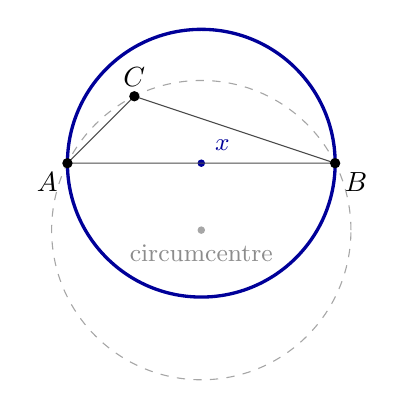
\begin{tikzpicture}[scale=0.85]
    \coordinate (A) at (0,0);
    \coordinate (B) at (4,0);
    \coordinate (C) at (1,1);
    \coordinate (O) at (2,-1);
    \coordinate (M) at (2,0);
    \draw[black!35, dashed] (O) circle (2.2360679);
    \fill[black!35] (O) circle (1.6pt);
    \node[black!45, below] at ($(O)+(0,-0.08)$) {\small circumcentre};
    \draw[blue!60!black, very thick] (M) circle (2);
    \fill[blue!60!black] (M) circle (1.6pt);
    \node[blue!60!black, above right] at ($(M)+(0.06,0.04)$) {\small $x$};
    \draw[black!70] (A) -- (B) -- (C) -- cycle;
    \foreach \P/\L/\pos in {A/A/below left, B/B/below right, C/C/above}
      { \fill (\P) circle (2.2pt); \node[\pos] at (\P) {$\L$}; }
  \end{tikzpicture}
  \end{center}

  This example is the whole difficulty of the problem in miniature. Fitting a
  circle \emph{through} a chosen set of points is easy linear algebra; the hard
  part is choosing the right set. Section~\ref{sec:algorithm} will show how the
  arithmetic itself tells us that $C$ has to go.
\end{example}

\section{Two convex formulations}
\label{sec:convex}

Problem~\eqref{eq:primal} is a convex optimisation problem: the objective $r$ is
linear and each constraint $\norm{p_i-x}\le r$ defines a convex set (a
second-order cone, in the joint variable $(r,x)$). So it can be handed to a
general-purpose conic solver, and the package accompanying these notes does
exactly that in one of its two solvers. But there is a second formulation that is
much closer to the geometry of Section~\ref{sec:certificate}, and it is the one
we will actually compute with.

\subsection{A quadratic program in the weights}

The certificate involved weights $w_j\ge0$ summing to one. Let us make those the
variables. Write
\[
  \simplex \;=\; \Bigl\{\, u \in \R^n \;:\; u_i \ge 0, \ \textstyle\sum_i u_i = 1 \,\Bigr\}
\]
for the unit simplex, and for $u\in\simplex$ define the \emph{weighted centre}
and the function
\begin{equation}
  \label{eq:phi}
  x(u) \;=\; \sum_{i=1}^n u_i p_i,
  \qquad
  \varphi(u) \;=\; \sum_{i=1}^n u_i \norm{p_i}^2 \;-\; \norm{x(u)}^2 .
\end{equation}
$\varphi$ is a \emph{concave} quadratic: the first term is linear in $u$ and the
second is a convex quadratic being subtracted. So maximising $\varphi$ over
$\simplex$ is a convex quadratic program --- and $\simplex$ is about the friendliest
feasible set there is.

The link to our problem is a single identity. For \emph{any} $y\in\R^d$ and any
$u\in\simplex$, expanding as in~\eqref{eq:parallel-axis} gives
\begin{equation}
  \label{eq:identity}
  \sum_{i=1}^n u_i \norm{p_i - y}^2 \;=\; \varphi(u) \;+\; \norm{x(u) - y}^2 .
\end{equation}

\begin{proposition}[Weak duality]
  \label{prop:weak}
  If $B(y,r)$ encloses $S$ then $\varphi(u)\le r^2$ for every $u\in\simplex$.
\end{proposition}

\begin{proof}
  Each $\norm{p_i-y}^2 \le r^2$, so the left side of~\eqref{eq:identity} is a
  weighted average of numbers no larger than $r^2$ and hence at most $r^2$. The
  right side is at least $\varphi(u)$.
\end{proof}

So every choice of weights produces a \emph{lower bound} $\sqrt{\varphi(u)}$ on
the optimal radius, and every enclosing ball produces an \emph{upper bound}. The
certificate of Section~\ref{sec:certificate} is exactly the statement that the two
bounds can be made to meet.

\begin{theorem}[Strong duality]
  \label{thm:strong}
  Let $R$ be the optimal radius. Then
  \[
    R^2 \;=\; \max_{u\in\simplex} \varphi(u),
  \]
  and if $w$ is a maximiser then $x=x(w)$ is the optimal centre.
\end{theorem}

\begin{proof}
  ``$\ge$'' is Proposition~\ref{prop:weak}. For ``$\le$'', take the optimal
  $B(x,R)$ and the certificate weights $w$ of Proposition~\ref{prop:necessary},
  padded with zeros so that $w\in\simplex$. Then $x(w)=x$, and
  putting $y=x$ in~\eqref{eq:identity} gives
  $\varphi(w) = \sum_i w_i\norm{p_i-x}^2 = R^2$, because $w_i>0$ only for support
  points, which are at distance exactly $R$. For the last claim, suppose
  $\varphi(w) = R^2$; taking $y=x$ in~\eqref{eq:identity} and using
  $\sum_i w_i \norm{p_i - x}^2 \le R^2$ forces $\norm{x(w)-x}^2 \le 0$.
\end{proof}

\begin{remark}
  Readers who have met Lagrangian duality will recognise $\varphi$ as the dual
  function of~\eqref{eq:primal} and the $u_i$ as the multipliers of the
  constraints $\norm{p_i-x}\le r$. Readers who have not have lost nothing: every
  statement above was proved with the identity~\eqref{eq:identity} and one line of
  algebra. The weights have a perfectly concrete meaning --- $u_i$ is how hard
  point $i$ pulls on the centre, and $u_i=0$ means it is not pulling at all.
\end{remark}

\subsection{What optimality looks like in the weights}

Differentiating~\eqref{eq:phi} and using~\eqref{eq:identity},
\begin{equation}
  \label{eq:gradient}
  \frac{\partial \varphi}{\partial u_i}(u)
    \;=\; \norm{p_i}^2 - 2\, x(u)\transpose p_i
    \;=\; \norm{p_i - x(u)}^2 - \norm{x(u)}^2 .
\end{equation}
The optimality conditions for maximising a concave function over the simplex say
that at a maximiser $w$ there is a number $\lambda$ with
\[
  \frac{\partial \varphi}{\partial u_i}(w) = \lambda \quad\text{whenever } w_i>0,
  \qquad
  \frac{\partial \varphi}{\partial u_i}(w) \le \lambda \quad\text{whenever } w_i=0 .
\]
Substituting~\eqref{eq:gradient} and cancelling the common $\norm{x}^2$, these read
\begin{equation}
  \label{eq:kkt}
  \norm{p_i - x} = R \ \text{ for all } i \text{ with } w_i>0,
  \qquad
  \norm{p_i - x} \le R \ \text{ for all } i \text{ with } w_i = 0 .
\end{equation}
Which is the geometric certificate, word for word: \emph{the points carrying
weight are on the boundary, and everything else is inside}. The optimisation and
the geometry are two descriptions of one object, and the algorithm below can be
read in either language.

\section{The active-set algorithm}
\label{sec:algorithm}

Corollary~\ref{cor:caratheodory} says the answer is determined by at most $d+1$
points. If we knew which ones, we could finish in a single linear solve. We do
not, so we guess and correct. That is the whole idea.

\subsection{The state}

The algorithm carries a \emph{working set} (or \emph{support set}) $F\subseteq
\{1,\dots,n\}$ of indices --- the current guess at which points touch the
boundary --- together with weights $u_i>0$ for $i\in F$ summing to one. In the
language of Section~\ref{sec:convex}, we are running an active-set method on the
QP $\max_{\simplex}\varphi$: the variables in $F$ are free and all others are
pinned at $u_i=0$.

\subsection{The subproblem: fit a ball to the working set}

Fix $F$ with points $q_0,\dots,q_{m-1}$. Ignore the other points entirely and
solve the equality-constrained subproblem: maximise $\varphi$ over weights
supported on $F$ and summing to one, with no sign restriction. By the same
computation that produced~\eqref{eq:kkt} --- but now with no inequality
multipliers, because there are no inequalities left --- a stationary point is
characterised by
\[
  \norm{q_j - x} \ \text{equal for all } j, \qquad x \in \aff\{q_0,\dots,q_{m-1}\} .
\]
So the subproblem is a piece of classical geometry: \emph{find the point in the
affine hull of the working set that is equidistant from all of them}, i.e.\ the
circumcentre of the face.

Parametrise the affine hull by the edge vectors $e_j = q_j - q_0$, $j=1,\dots,m-1$,
collected as the rows of the $(m-1)\times d$ matrix $D$, and write
$x = q_0 + D\transpose y$. Then
\[
  \norm{x-q_j}^2 = \norm{x-q_0}^2
  \iff -2\,e_j\transpose(x-q_0) + \norm{e_j}^2 = 0
  \iff \bigl(D D\transpose y\bigr)_j = \tfrac12 \norm{e_j}^2 .
\]
This is an $(m-1)\times(m-1)$ system with the Gram matrix $DD\transpose$, which is
positive definite exactly when the edges are linearly independent --- that is,
when $q_0,\dots,q_{m-1}$ are \emph{affinely independent}. Since $m\le d+1$ in the
cases we care about, this is a very small dense solve. Converting back to weights,
\begin{equation}
  \label{eq:face-weights}
  w = \Bigl(1 - \textstyle\sum_j y_j,\ y_1,\ \dots,\ y_{m-1}\Bigr),
  \qquad x = \sum_j w_j q_j .
\end{equation}

\subsection{Reading the signs}

The subproblem ignored the constraint $u\ge0$, so its answer may violate it, and
that is exactly the information we need.

\begin{itemize}
  \item \textbf{All $w_j \ge 0$.} The circumcentre lies inside the region spanned
    by the working set, so half the certificate~\eqref{eq:kkt} already holds: the
    points of $F$ are on the boundary and surround the centre. Accept the step
    and go check the other half.
  \item \textbf{Some $w_j < 0$.} The circumcentre has fallen \emph{outside} the
    working set's convex hull --- Example~\ref{ex:obtuse} is precisely this
    situation, with $w_C=-1$. That point is not holding the ball out; it is being
    dragged along. Rather than jumping to an infeasible $w$, move from $u$ towards
    $w$ and stop the moment the first weight reaches zero:
    \begin{equation}
      \label{eq:ratio}
      \alpha = \min\Bigl\{\, \frac{-u_i}{s_i} \;:\; s_i < 0 \,\Bigr\},
      \qquad s = w - u,
      \qquad u \leftarrow u + \alpha s .
    \end{equation}
    Drop the index that hit zero from $F$ and repeat. This is the classical
    \emph{ratio test} of active-set methods, and here it has a plain geometric
    reading: eject the point that stopped touching the boundary.
\end{itemize}

\subsection{Growing the working set}

Suppose the subproblem gave a feasible $w$, with centre $x$ and radius $R$. Sweep
\emph{all} $n$ points and compare. If $\norm{p_i-x}\le R$ for every $i$, then
by~\eqref{eq:kkt} --- or directly by Theorem~\ref{thm:sufficient} --- we are done
and the answer is exact. Otherwise pick the worst offender,
\[
  k \;=\; \argmax_i \norm{p_i - x}^2 ,
\]
add $k$ to $F$ with initial weight $0$, and repeat. Adding the \emph{farthest}
violator is the greedy choice: it is the point in most urgent need of covering,
and by~\eqref{eq:gradient} it is also the free variable with the largest
improvement in $\varphi$, so it is steepest ascent as well as common sense.

\subsection{The degenerate case}

One case remains. The working set can become affinely \emph{dependent} --- three
collinear points in the plane, or any $d+2$ points --- and then the Gram matrix
$DD\transpose$ is singular and there is no unique circumcentre to jump to.

Look at what that means for $\varphi$. A weight direction $s$ satisfying
\[
  \sum_i s_i = 0 \qquad\text{and}\qquad \sum_i s_i q_i = 0
\]
moves the weights without moving the centre $x(u)$ at all. Eliminating
$s_0 = -\sum_{j\ge1}s_j$ turns the second condition into $D\transpose s_{1:} = 0$,
so such directions exist precisely when $D$ has a non-trivial left null space,
i.e.\ precisely when the face is affinely dependent. Along any of them the term
$\norm{x(u)}^2$ in~\eqref{eq:phi} is frozen, so
\[
  \varphi(u + t s) = \varphi(u) + t \sum_i s_i \norm{p_i}^2
\]
is \emph{linear} in $t$: the subproblem is unbounded, and the right response is
not to jump anywhere but to slide. Project the gradient~\eqref{eq:gradient} onto
the null space, follow it, and apply the same ratio test~\eqref{eq:ratio}. A
weight is driven to zero, the working set shrinks by one, and affine independence
is restored.

\subsection{The algorithm, assembled}

\begin{center}
\fbox{\begin{minipage}{0.92\textwidth}
\textbf{Active-set method for the smallest enclosing ball}\\[0.4em]
\emph{Input:} points $p_1,\dots,p_n \in \R^d$. \emph{Output:} $R$, $x$, weights $u$.
\begin{enumerate}\itemsep2pt
  \item Recentre: replace $p_i$ by $p_i - \bar p$ (undo at the end).
  \item Initialise $F=\{k\}$ where $k$ is the point farthest from $p_1$, and $u_k=1$.
  \item \textbf{repeat}
  \begin{enumerate}\itemsep2pt
    \item If the face $\{p_i\}_{i\in F}$ is affinely \emph{dependent}: compute a
      descent direction $s$ in the null space, take the ratio
      step~\eqref{eq:ratio}, drop a zero weight, and continue.
    \item Otherwise solve~\eqref{eq:face-weights} for the circumcentre weights $w$.
    \item If $\min_j w_j < 0$: set $s = w-u$, take the ratio step~\eqref{eq:ratio},
      drop a zero weight, and continue.
    \item Otherwise accept $u \leftarrow w$, $x \leftarrow x(u)$,
      $R \leftarrow \max_{i\in F}\norm{p_i-x}$.
    \item Let $k = \argmax_i \norm{p_i-x}$. If $\norm{p_k-x}\le R$: \textbf{return}
      $(R,\, x+\bar p,\, u)$.
    \item Otherwise drop the zero weights from $F$, append $k$ with weight $0$.
  \end{enumerate}
\end{enumerate}
\end{minipage}}
\end{center}

\begin{example}[Example~\ref{ex:obtuse} by hand]
  Start with $F=\{A,B\}$ (the two farthest-apart points). The circumcentre of two
  points is their midpoint $(2,0)$ with weights $(\tfrac12,\tfrac12)\ge0$, so
  $R=2$. Sweep: $\norm{C-(2,0)}=\sqrt2 < 2$, so nothing is outside and we return
  immediately.

  Start instead with $F=\{A,C\}$ to see the interesting branch. The midpoint is
  $(0.5,0.5)$ with $R=\sqrt{0.5}\approx0.707$; the farthest point is $B$, at
  distance $\approx3.54$, so $B$ joins and $F=\{A,C,B\}$. The circumcentre
  of the three is $(2,-1)$ with weights $(1.25,\,-1,\,0.75)$ --- negative on $C$.
  The ratio test~\eqref{eq:ratio} moves as far as it can and drops $C$, leaving
  $F=\{A,B\}$, and the next iteration returns $R=2$, $x=(2,0)$ as before.
\end{example}

\subsection{Why it terminates, and how fast}

\paragraph{Termination.} Each iteration either strictly increases $\varphi$ or
strictly shrinks the working set, and there are finitely many working sets, so the
method cannot wander forever. Two remarks are in order. First, this is the
standard finite-termination argument for active-set methods, and like all of them
it has a caveat: a degenerate step of length $\alpha=0$ makes no progress in
$\varphi$, and in exact arithmetic one needs an anti-cycling rule (Bland's, say)
to rule out an infinite loop. In practice implementations use an iteration cap as
a safety net and never hit it. Second, when the method stops it stops at an
\emph{exact} vertex-like configuration --- a specific working set with a specific
linear solve --- not at a tolerance. On inputs whose answer is exactly
representable, it returns that answer bit for bit.

\paragraph{Cost.} Per iteration:
\begin{itemize}
  \item one sweep of squared distances over all points, $O(nd)$, which vectorises
    perfectly;
  \item one Gram matrix and dense solve of size $m-1 \le d$, so $O(m^2 d + m^3)$.
\end{itemize}
Note what is \emph{not} there: no factorisation of anything of size $n$. The
linear algebra is governed by the ambient dimension, and $n$ enters only through
one streaming pass. This is the structural reason the method scales far better in
$n$ than a general conic solver, which must factor an $n$-row constraint matrix at
every interior-point iteration. Empirically the number of iterations is a small
multiple of the final support size; the classical worst-case analyses and the
expected-time results for randomised variants are in the references
(\S\ref{sec:notes}).

\section{Making it numerically honest}
\label{sec:numerics}

The mathematics above is exact. Floating point is not, and a naive transcription
fails on inputs that are geometrically unremarkable. Four points are worth
knowing; all four are consequences of one principle: \emph{no tolerance may
secretly assume that the coordinates are of size~$1$.}

\paragraph{Recentre first.} Replace $p_i$ by $p_i-\bar p$ before doing anything.
Otherwise consider a cloud of extent $1$ sitting a million units from the origin:
the squared coordinates are of size $10^{12}$, their rounding error is of size
$10^{12}\varepsilon \approx 10^{-4}$, and the radius we are trying to resolve is of
size $1$. Every quantity in the algorithm --- Gram matrix, distances, rounding
floor --- should be governed by the \emph{extent} of the cloud, never by its
distance from an arbitrary origin. Recentring costs one pass and buys exactly
that. The result is that the answer is invariant under translation of the input,
as of course it must be mathematically.

\paragraph{Difference before you square.} Compute $\norm{p-x}^2$ as
$\sum_k (p_k-x_k)^2$, never as $\norm{p}^2 - 2p\transpose x + \norm{x}^2$. The
second form subtracts quantities of size $\norm{x}^2$ from each other to produce
an answer of size $R^2$, and every digit by which $\norm{x}$ exceeds $R$ is a
digit lost to cancellation. The first form has no cancellation at all.

\paragraph{Test rank on the edges.} The affine-dependence test of
Section~\ref{sec:algorithm} is a rank test. It is tempting to run it on the
stacked matrix $\begin{psmallmatrix}\mathbf{1}\transpose\\ Q\transpose\end{psmallmatrix}$,
which encodes ``sums to zero and fixes the centre'' in one go. Do not: the row of
ones has entries of size $1$, so it dominates the singular values, and any cloud
whose extent is small relative to $1$ is then declared degenerate whatever its
actual geometry. Eliminating the sum constraint by hand and testing the rank of the
edge matrix $D$ --- as in Section~\ref{sec:algorithm} --- keeps the test
scale-invariant.

\paragraph{Size the tolerances in the right units.} The stopping test
``is any point outside?'' compares squared distances, which carry units of
length$^2$. A relative tolerance handles the ordinary case; but near the
degenerate limit one also needs an absolute floor, and that floor must be
proportional to $\varepsilon \max_i \norm{p_i}^2$ rather than a fixed constant. The
same applies to the null-space direction of the degenerate branch: the gradient
carries units of length$^2$, so normalise the direction to unit maximum before
comparing anything derived from it against a dimensionless weight tolerance.
Otherwise, on a cloud of extent $10^{-20}$, no component ever looks binding.

Both invariances --- under translation and under scaling --- deserve explicit
regression tests, since they are easy to break with a well-meant simplification
and produce plausible-looking wrong answers rather than crashes.

\section{Using the code}
\label{sec:code}

These notes accompany \texttt{cvxball}, which ships the active-set method of
Section~\ref{sec:algorithm} and nothing else: NumPy is its only dependency. The
second-order cone program of Section~\ref{sec:convex} is implemented too, but
under \texttt{experiments/}, where it is what it has in fact become --- the
reference the shipped method is measured against, sharing its interface so the
two can be tested against each other.

\begin{lstlisting}
import numpy as np
from cvxball import min_circle_active_set
from experiments.clarabel_ball import min_circle_clarabel   # reference

points = np.array([[0.0, 0.0], [4.0, 0.0], [1.0, 1.0]])

radius, centre = min_circle_active_set(points)   # -> 2.0, array([2., 0.])
radius, centre = min_circle_clarabel(points)     # the same, to solver tolerance
\end{lstlisting}

The correspondence with the text is direct:

\begin{center}
\begin{tabular}{ll}
  \toprule
  \textbf{In these notes} & \textbf{In the source} \\
  \midrule
  Subproblem~\eqref{eq:face-weights}, the circumcentre & \texttt{\_face\_weights} \\
  Affine-dependence test and null space  & \texttt{\_affine\_null\_space} \\
  Squared distances, differenced         & \texttt{\_sq\_dist} \\
  The main loop                          & \texttt{min\_circle\_active\_set} \\
  The cone program of \S\ref{sec:convex} & \texttt{experiments/clarabel\_ball.py} \\
  Welzl's algorithm, for comparison      & \texttt{experiments/welzl.py} \\
  Conic front end, \S\ref{sec:frontend} & \texttt{cvxball.active\_set.DefaultSolver} \\
  Goldfarb--Idnani QP, \S\ref{sec:gi}   & \texttt{cvxball.qp.solve\_qp} \\
  \bottomrule
\end{tabular}
\end{center}

A third entry point, \texttt{cvxball.active\_set}, wraps the same method in the
interface of a general-purpose solver; that is the subject of
Section~\ref{sec:frontend}.

The optimal weights $u$ of Theorem~\ref{thm:strong} are more than a by-product:
they are the certificate. Given $(R,x,u)$ a sceptic can verify optimality without
re-running anything --- check $u\ge0$, check $\sum_i u_i = 1$, check
$x=\sum_i u_i p_i$, check $\norm{p_i-x}\le R$ for all $i$ with equality wherever
$u_i>0$ --- and Theorem~\ref{thm:sufficient} then guarantees the answer. Verifying
a solution is cheaper than finding one, which is a good habit to acquire early.

\section{The same idea in a solver's clothing}
\label{sec:frontend}

Everything so far has been about one specific problem. This last section shows
what happens when you package the method as a \emph{solver} --- something that
accepts a problem in a standard form rather than a point cloud --- and what the
weights of Theorem~\ref{thm:strong} turn into when you do. Nothing new is
proved here; the point is that the objects we built by hand are the objects the
general theory already had names for.

\subsection{Conic standard form}
\label{sec:conic}

A conic program is written
\begin{equation}
  \label{eq:conic}
  \text{minimise}\quad \tfrac12 z\transpose P z + q\transpose z
  \qquad\text{subject to}\qquad
  A z + s = b, \quad s \in \mathcal{K},
\end{equation}
where $\mathcal{K}$ is a product of simple convex cones. Three kinds cover most
of what one meets:
\begin{center}
\begin{tabular}{lll}
  \toprule
  \textbf{Cone} & \textbf{Definition} & \textbf{What it expresses} \\
  \midrule
  zero cone            & $\{0\}$ & an equality row $a\transpose z = b$ \\
  non-negative orthant & $\{s : s\ge 0\}$ & an inequality row $a\transpose z \le b$ \\
  second-order cone $\mathcal{Q}^{k+1}$ & $\{(t,v)\in\R\times\R^k : \norm{v}\le t\}$
    & a Euclidean norm bound \\
  \bottomrule
\end{tabular}
\end{center}

The slack variable $s$ is what the constraint leaves over, and requiring
$s\in\mathcal{K}$ is what makes it a constraint. Our
problem~\eqref{eq:primal} fits with no cleverness at all. Take the decision
vector $z=(r,x_1,\dots,x_d)$, minimise $r$ (so $P=0$ and $q$ is the first unit
vector), and note that
\[
  \norm{p_i - x} \le r
  \quad\Longleftrightarrow\quad
  s_i := (r,\; p_i - x) \in \mathcal{Q}^{d+1} .
\]
One second-order cone per point, each of dimension $d+1$, stacked into one $A$
and one $b$. That is the whole translation, and it is what
\texttt{\_build\_soc\_program} performs.

\subsection{The weights, in the solver's coordinates}

A conic solver is expected to return not just the primal $z$ but a \emph{dual}
vector $\zeta$, one block per cone, certifying optimality. For the ball problem
we already have a certificate --- the weights $u$ --- so the two had better be
the same object. They are, after one change of coordinates: point $i$'s block is
\begin{equation}
  \label{eq:conic-dual}
  \zeta_i \;=\; u_i \left(1,\; -\frac{p_i - x}{R}\right) .
\end{equation}
Two lines of arithmetic show this is exactly what the theory asks for.

\emph{It lies in the cone.} The tail of $\zeta_i$ has norm
$u_i\norm{p_i-x}/R$, which for a support point ($\norm{p_i-x}=R$) equals $u_i$,
its head. So $\zeta_i$ sits on the \emph{boundary} of $\mathcal{Q}^{d+1}$ for
every support point, and is the zero vector for every other point.

\emph{It is complementary to the slack.} Pair $\zeta_i$ with the slack
$s_i=(R,\,p_i-x)$ of Section~\ref{sec:conic}:
\[
  s_i\transpose \zeta_i
    \;=\; u_i\left(R - \frac{\norm{p_i-x}^2}{R}\right)
    \;=\; \frac{u_i}{R}\Bigl(R^2 - \norm{p_i-x}^2\Bigr) \;=\; 0 ,
\]
because each factor kills the other: where $u_i>0$ the point is on the boundary
and the bracket vanishes; where the bracket does not vanish, $u_i=0$. This is
\emph{complementary slackness}, and comparing it with~\eqref{eq:kkt} shows it is
the certificate of Section~\ref{sec:certificate} written in the solver's
alphabet. The geometry (\emph{which points touch}), the optimisation (\emph{which
multipliers are non-zero}) and the conic algebra (\emph{which blocks are on the
cone boundary}) are three vocabularies for one fact.

\begin{remark}
  This is why an implementation should keep the weights rather than discard
  them. Returning $(R,x)$ answers the question; returning $(R,x,u)$ lets the
  caller \emph{check} the answer, and --- via~\eqref{eq:conic-dual} --- hands a
  conic solver's caller the dual it expects, at no extra cost.
\end{remark}

\subsection{The general quadratic program}
\label{sec:gi}

Once the front door accepts~\eqref{eq:conic}, most incoming problems are not
enclosing balls. If every cone is a zero cone or an orthant, \eqref{eq:conic} is
an ordinary convex quadratic program,
\begin{equation}
  \label{eq:qp}
  \text{minimise}\quad \tfrac12 x\transpose P x + q\transpose x
  \qquad\text{subject to}\qquad E x = f, \quad G x \le h,
\end{equation}
with $P$ symmetric positive definite. The same active-set idea applies, in the
form given by Goldfarb and Idnani~\cite{goldfarb1983}, and it is instructive to
see how little changes:
\begin{itemize}
  \item \textbf{Working set.} A guess at which of the inequality rows of $G$ are
    tight at the optimum --- the analogue of the support set.
  \item \textbf{Subproblem.} Minimise the objective subject to the working-set
    rows holding as \emph{equalities}. That is one $k\times k$ dense solve with
    $k$ the size of the working set --- the analogue
    of~\eqref{eq:face-weights}.
  \item \textbf{Drop.} If a multiplier would go negative, that row is not really
    pushing; ratio-test to the boundary and drop it --- the analogue
    of~\eqref{eq:ratio}.
  \item \textbf{Add.} Otherwise scan all the rows and add the most violated one
    --- the analogue of adding the farthest point.
\end{itemize}

The one genuinely new idea is the choice of the word \emph{dual} in ``dual
active-set method''. A \emph{primal} method must start from a feasible point, and
finding one is a separate optimisation problem in its own right (``phase one'').
Goldfarb--Idnani sidesteps this: it starts at the unconstrained minimiser
$x=-P^{-1}q$, which is always available and needs only one Cholesky
factorisation, and it adds constraints one at a time while keeping every
multiplier non-negative. Feasibility is what it works \emph{towards}; optimality
of the current working set is the invariant it never gives up. This is why the
enclosing-ball method of Section~\ref{sec:algorithm} could also begin anywhere it
liked --- with a single point --- and still be correct at every step.

\begin{remark}[On not answering a different question]
  The method above needs $P\succ0$; the subproblem is otherwise not a minimum.
  A tempting shortcut is to add $\epsilon I$ to any $P$ until it factorises. For
  a $P$ that is positive semidefinite but numerically borderline that is a fair
  regularisation. For a genuinely \emph{indefinite} $P$ it is not: the true
  problem has no minimum, and $P+\epsilon I$ silently replaces it with a
  convexified one whose answer is unrelated. Refusing is the honest response,
  and a solver that returns a confident number for an ill-posed question is worse
  than one that declines.
\end{remark}

\subsection{Why bother, when interior-point methods exist}

Interior-point methods solve~\eqref{eq:conic} well and are the right tool for
large sparse programs. The trade the active-set methods offer is different, and
worth stating plainly because it is the reason this package exists.

An interior-point method approaches the optimal face \emph{from the inside}. It
stops when a duality gap falls below a tolerance, at which point the constraints
that are ``really'' tight have slacks of perhaps $10^{-9}$ and the ones that are
not have slacks of $10^{-4}$, and the caller must decide where to draw the line.
An active-set method identifies the face \emph{combinatorially} --- a set of
indices --- and then solves that face exactly. If your question is
\emph{which} constraints bind (which holdings sit on their bound, which points
touch the sphere), one method returns a discrete answer and the other returns
numbers you must round. Per iteration the active-set method also factors nothing
of size $n$, which is what makes it scale in the number of constraints the way
Section~\ref{sec:algorithm} described.

\begin{remark}[A note on defensive programming]
  Recognising ``an enclosing-ball program'' by counting cones is not enough: a
  program can have $n$ second-order cones of dimension $d+1$ and still be some
  other problem entirely. The safe check is to reconstruct the point cloud from
  $(A,b)$, rebuild the program those points \emph{would} produce, and compare it
  with the one that arrived. A look-alike is then refused rather than answered
  with the solution to a problem nobody asked about.
\end{remark}

\section{Exercises}
\label{sec:exercises}

\begin{exercise}
  \label{ex:circum}
  Verify the claims of Example~\ref{ex:obtuse}: that the circle through
  $(0,0),(4,0),(1,1)$ has centre $(2,-1)$ and radius $\sqrt5$, and that the
  barycentric weights of that centre with respect to the three points are
  $(1.25,\,0.75,\,-1)$. Which sign told you the circumcircle was not the answer?
\end{exercise}

\begin{exercise}
  Prove that the smallest enclosing ball of $S$ equals the smallest enclosing ball
  of the vertices of $\conv S$. (Hence no interior point is ever a support point.)
\end{exercise}

\begin{exercise}
  Show that in the plane the support set of the optimal ball never consists of
  three points forming an obtuse triangle. Generalise: if three support points
  form a triangle with an obtuse angle at $q_j$, derive a contradiction with
  $x\in\conv T$.
\end{exercise}

\begin{exercise}
  Fill in the algebra of~\eqref{eq:identity}, and deduce
  Lemma~\ref{lem:shrink} from it by choosing $n=2$ and
  $u=(\tfrac12,\tfrac12)$ applied to the two \emph{centres}. (The shrinking lemma
  and the parallel-axis identity are the same fact.)
\end{exercise}

\begin{exercise}
  Let $S$ lie on a sphere of radius $\rho$ about the origin. Show
  $\varphi(u) = \rho^2 - \norm{x(u)}^2$, so that maximising $\varphi$ is the same
  as finding the point of $\conv S$ closest to the origin. Interpret the case
  $0\notin\conv S$.
\end{exercise}

\begin{exercise}
  Implement the algorithm from the box in Section~\ref{sec:algorithm} in fifty
  lines, ignoring all of Section~\ref{sec:numerics}. Then construct an input on
  which it fails: translate a unit-extent cloud far from the origin, and separately
  shrink one to extent $10^{-20}$. Explain each failure in terms of the four
  principles listed there.
\end{exercise}

\begin{exercise}
  Verify directly that the vector $\zeta_i$ of~\eqref{eq:conic-dual} satisfies
  $\norm{\text{tail}} \le \text{head}$ for \emph{every} $i$, not merely for the
  support points, so that $\zeta$ really is a point of the cone. Where in the
  argument did you use $\norm{p_i - x} \le R$?
\end{exercise}

\begin{exercise}
  Write the enclosing-ball problem in the form~\eqref{eq:qp} instead --- that is,
  as a quadratic program in the weights $u$ over the simplex, using
  Theorem~\ref{thm:strong}. What are $P$, $q$, $E$, $f$, $G$ and $h$? Is your $P$
  positive definite, and what does your answer mean for
  Section~\ref{sec:gi}?
\end{exercise}

\begin{exercise}
  The method as described adds one point per outer iteration. Suppose instead you
  add the $k$ farthest violators at once. Does the algorithm still terminate? Does
  the certificate check change? (This is the ``multiple pricing'' idea from linear
  programming.)
\end{exercise}

\section{Notes and further reading}
\label{sec:notes}

The problem is old: Sylvester posed the planar case in 1857~\cite{sylvester1857}.
Elzinga and Hearn~\cite{elzinga1972} gave an early finite algorithm of the type
developed here. Welzl's randomised incremental algorithm~\cite{welzl1991} runs in
expected $O(n)$ time for fixed $d$ and is beautifully short, though its recursion
degrades as $d$ grows. G\"artner~\cite{gaertner1999} made it robust.

From there the subject forks, and it is worth being clear about which branch this
is. The method of Section~\ref{sec:algorithm} is of the quadratic-programming
line --- G\"artner and Sch\"onherr~\cite{gaertner2000} --- whose state is the
weight vector of Section~\ref{sec:convex} and whose every pivot solves the face
exactly. Fischer, G\"artner and Kutz~\cite{fischer2003} take the other branch:
they keep a pair (support set, centre) and \emph{walk} the centre towards the
circumcentre, stopping the moment a new point catches the shrinking sphere, so
their iterate is in general not a circumcentre at all. They also supply what
Section~\ref{sec:algorithm} only gestured at --- an explicit Bland-type order on
the points, with a proof that it terminates --- and then note that it is too slow
to use in practice. Their reservation about QP formulations, that robustness past
a few hundred dimensions demanded exact arithmetic, is worth carrying alongside
Section~\ref{sec:numerics}: the invariances there are an answer to that concern,
not evidence against it.

The active-set machinery --- working sets, ratio tests, dropping constraints ---
is standard quadratic programming; Goldfarb and Idnani~\cite{goldfarb1983} is the
canonical dual method and Nocedal and Wright~\cite{nocedal2006} the standard
textbook treatment. For the convex-analytic background, including conic
formulations and duality done properly, see Boyd and
Vandenberghe~\cite{boyd2004}, which is freely available.

A last word on what this problem teaches. Almost every idea here recurs: a
certificate that is cheaper to check than to find; an optimality condition that
reads simultaneously as geometry and as calculus; an algorithm that guesses the
combinatorial structure and repairs it; and a numerical implementation whose
tolerances must be dimensionally honest. The smallest enclosing ball is small
enough to hold in your head and rich enough to contain all four.

\begin{thebibliography}{9}
\bibitem{boyd2004}
  S.~Boyd and L.~Vandenberghe.
  \emph{Convex Optimization}.
  Cambridge University Press, 2004.

\bibitem{elzinga1972}
  J.~Elzinga and D.~W.~Hearn.
  Geometrical solutions for some minimax location problems.
  \emph{Transportation Science} 6(4):379--394, 1972.

\bibitem{fischer2003}
  K.~Fischer, B.~G\"artner and M.~Kutz.
  Fast smallest-enclosing-ball computation in high dimensions.
  In \emph{Proc.\ 11th European Symposium on Algorithms (ESA)}, 630--641, 2003.

\bibitem{gaertner1999}
  B.~G\"artner.
  Fast and robust smallest enclosing balls.
  In \emph{Proc.\ 7th European Symposium on Algorithms (ESA)}, 325--338, 1999.

\bibitem{gaertner2000}
  B.~G\"artner and S.~Sch\"onherr.
  An efficient, exact, and generic quadratic programming solver for geometric
  optimization.
  In \emph{Proc.\ 16th Annual ACM Symposium on Computational Geometry},
  110--118, 2000.

\bibitem{goldfarb1983}
  D.~Goldfarb and A.~Idnani.
  A numerically stable dual method for solving strictly convex quadratic programs.
  \emph{Mathematical Programming} 27:1--33, 1983.

\bibitem{nocedal2006}
  J.~Nocedal and S.~J.~Wright.
  \emph{Numerical Optimization}, 2nd edition.
  Springer, 2006.

\bibitem{sylvester1857}
  J.~J.~Sylvester.
  A question in the geometry of situation.
  \emph{Quarterly Journal of Pure and Applied Mathematics} 1:79, 1857.

\bibitem{welzl1991}
  E.~Welzl.
  Smallest enclosing disks (balls and ellipsoids).
  In \emph{New Results and New Trends in Computer Science}, LNCS 555, 359--370, 1991.
\end{thebibliography}

\end{document}
